\chapter{File Systems and Storage Devices}
\label{chap:file_system}

In computing, a {\bf file system} (or filesystem) controls how data is stored or
retrieved on a persistent memory storage (e.g. harddisk, tapes, \ldots). There
are many different kinds of file systems (Sect.\ref{sec:file_system}). One file
system can be deployed on many different kinds of persistent storage devices
(Sect.\ref{sec:storage_devices}); and each storage device can be configured to
use with different kinds of file systems.

\section{Storage devices}
\label{sec:storage_devices}

\subsection{hard drive}

The most common storage device is the {\bf hard drive}, a disc coated with a
magnetic film. The film has ones and zeross 'writen' on it sending electrical
pulses to a magnetic 'read-write' head.

\subsection{magnetic tape}

\subsection{optical disc}

\subsection{flash memory}

\section{Storage Virtualization}
\label{sec:storage_virtualization}

One of the real contributions of Unix has been the view that "everything is a
file". In Linux, a hardware device, including storage device, is identified as a single
file in \verb!/dev/! folder. Typically, the O/S sees each storage device 
limited by its capacity.
{\bf Virtualization} enables combining multiple physical storage devices into a
single 

\section{File System}
\label{sec:file_system}

A file system is a {\bf low-level software layer} that handles writing/reading
data to a particular storage device. The implementation determines how data are
stored and retrieved on the storage device.

It allows the operating system to be 'free' from the underlying
hardware/software architecture of the storage device. Example: the O/S call the
same API, regardles of the data being sent to the printer, or a hard-disk.

There are so many different types of file systems. Typically, file system refers
to the software layer handling data write/read from a hard-disk. However, we
also have virtual file system (Sect.\ref{sec:filesystem-virtual}).

For a hard-disk, without a file system, information placed in a storage area
would be one large body of data with no way to tell where one piece of
information stops and the next begins.
\begin{itemize}
  \item  Frequently retail systems are configured with a single file system
  occupying the entire hard disk. 

  \item Another approach is to partition the disk so that several file
systems with different attributes can be used.

  \item A third approach, which is mostly used in cloud systems, is to use "disk
images" to house additional file systems, with the same attributes or not, within
another (host) file system as a file, e.g. 

\begin{itemize}
  \item virtualization: one runs an experimental Linux distribution (using ext4
  file system) in a virtual machine under the production Windows environment
  (using NTFS file system). Here, the ext4 file system resides in a disk image
  treated as a single file (or multiple files, depending on the hypervisor and
  settings) in the NTFS host file system.
\end{itemize}

\end{itemize}

Many file systems adress data based on the physical address on the disk; so it
is limited to a single disk, i.e. data can not spread onto 2 different disks.
Different operating systems (Windows, Linux, \ldots), depending on its version,
can use a different file system.

\subsection{Block-oriented file system}
\label{sec:filesystem_block-oriented}

Disk file systems are usually block-oriented. Files in a block-oriented file
system are sequences of blocks, often featuring fully random-access read, write,
and modify operations. 

\begin{itemize}
  \item FAT (FAT12, FAT16, FAT32)
  \item exFAT
  \item NTFS
  \item HFS
  \item HFS+
  \item HPFS
  \item UFS
  \item ext2, ext3, ext4 - Sect.\ref{sec:ext2}
  \item XFS
  \item btrfs
  \item ISO 9660
  \item Veritas File System
  \item VMFS
  \item ZFS
  \item ReiserFS
  \item UDF
\end{itemize}

A file system should contains the following information
\begin{itemize}
  \item rules to define a file name (e.g. no longer than 14 characters or 8.3
  filenames)
  
  \item maximum file size. The first Linux file system, {\it Minix} defines
  maximum 64MB per file.
  
  \item rule to define size for data blocks
  (Sect.\ref{sec:block-size-in-a-block-oriented-filesystem}). 
  
  \item {\bf inode data structure} for each file: Sect.\ref{sec:inode-in-a-block-oriented-filesystem}
    
NOTE: The inodes for the file system are all kept together in inode tables.
  
  \item what is a folder? -
  Sect.\ref{sec:folder-in-a-block-oriented-filesystem}
    
  \item some other advanced features: fault-tolerance \ldots
\end{itemize}
\url{http://www.tldp.org/LDP/tlk/fs/filesystem.html}


Some disk file system are aka
\begin{itemize}
  \item journaling file systems
  \item versioning file systems
\end{itemize} 



\subsection{-- block}
\label{sec:block-size-in-a-block-oriented-filesystem}

In block-oriented file systems, depending on the file system being used, the
disk is configured in \textcolor{red}{blocks of a fixed sizes}, e.g. 4KB, 8KB.

In EXT2, these data blocks are all of the same length and, although that
length can vary between different EXT2 file systems the block size of a
particular EXT2 file system is set when it is created (using \verb!mke2fs!).

Every file's size is rounded up to an integral number of blocks. If the block
size is 1024 bytes, then a file of 1025 bytes will occupy two 1024 byte blocks.
  
In the beginning, the disk is blank, and it needs to be configured (e.g. using
\verb!fdisk!) with
\begin{itemize}
  \item partition structure: to divide the physical disk into a number of
  logical partitions
  \item configure and create the file system for each partition (or the whole
  disk). File systems organize files into logical hierarchical structures with
  directories, soft links and so on held in data blocks on physical
  storage devices
\end{itemize}
In Linux, devices that can contain file systems are known as block devices. 


\subsection{-- metadata}
\label{sec:metadata-in-a-block-oriented-filesystem}

A file system keeps the metadata structure that can help to tell the
locations of all data blocks of a file.

RESTRICTION: \textcolor{red}{A single block can only contains data from one
file}, i.e. if a system has lots of small files, it's suggested to use small
block size for storage efficiency. The related files can be organized under the
same 'namespace', called {\it folder}. This hierachical structure is organized
and managed by the file system as metadata.

The metadata is often organized in the form of some tree-like data structure,
e.g. B-tree, H-tree,\ldots for fast indexing. 


\subsection{-- inode}
\label{sec:inode-in-a-block-oriented-filesystem}

The inodes for the file system are all kept together in inode tables.

An inode describes which blocks the data within a file occupies as well as the
access rights of the file, the file's modification times and the type of the
file.

\subsection{-- file}
\label{sec:file-in-a-block-oriented-filesystem}

The data are stored in a number of blocks
(Sect.\ref{sec:block-size-in-a-block-oriented-filesystem}), these blocks are
group under the name 'file'.

Every file in the EXT2 file system is described by a single inode
(Sect.\ref{sec:inode-in-a-block-oriented-filesystem}) and each inode has a
single unique number identifying it.


\subsection{-- folder}
\label{sec:folder-in-a-block-oriented-filesystem}

In EXT2 file system, a folder is a special file
(Sect.\ref{sec:file-in-a-block-oriented-filesystem}), whose content are pointers
pointing to the inodes (Sect.\ref{sec:inode-in-a-block-oriented-filesystem})
holding the folder's directory and file entries.

\subsection{-- data integrity}
\label{sec:data-integrity-in-a-block-oriented-filesystem}

File system integrity checking is important to ensure data are not lost, i.e. no
data corruption.
\begin{enumerate}
  \item ext2: only check at the boot-time
  
  \item ext3, ext4: maintained continuously during normal operation 
  
  
NOTE: It can be forced to check filesystem integrity using \verb!fsck! command.
  
\end{enumerate}

\subsection{-- ext2, ext3, ext4}
\label{sec:EXT2}
\label{sec:EXT3}
\label{sec:EXT4}

File system integrity is maintained continuously during normal operation in the
ext3 and ext4 file systems.

If the disk is larger than 6GB, then don't use EXT2 as it requires periodic file
system integrity checking (which takes boot-up longer for large partition). 

The main tool for checking file system is \verb!fsck!.



\subsection{Record-oriented file systems}
\label{sec:filesystem_record-oriented}

This is often used in mainframe and minicomputer O/S. In record-oriented file
systems files are stored as a collection of records.

Each record, by itself, is a completed set of data as a whole. This is popular
in banking.

\begin{itemize}
  \item Files-11
  \item MTS
  \item OS4000
  \item POS (Pick Operating System)
  \item RSD (Record Sequential Delimited)
  \item SFS (Structured File Server)
  \item VSAM (Virtual Storage Access Method)
\end{itemize}



\section{Scalable file systems}
\label{sec:filesystem-scalable}

Each file system (Sect.\ref{sec:file_system}) has some functional limit that
defines the maximum storable data capacity within that system.

\subsection{Shared-disk file systems}
\label{sec:filesystem-scalable-shared-disk}

Other names: shared-storage file systems, SAN file system, Clustered file system
or even cluster file systems. SAN = storage area network, where all nodes
directly access the block storage where the file system is located. 

Shared-disk file systems are normally used in a high-availability cluster
together with storage on hardware RAID. Shared-disk file systems normally do not
scale over 64 or 128 nodes. 

To keep the information of data in different nodes, the metadata can be stored 
in a centralized metadata servers (asymmetric), or distributed among the nodes
(symmetric).

\subsection{Distributed file systems}
\label{sec:distributed_filesystem}
\label{sec:filesystem-scalable-distributed}

%Other names: network file systems (NFS). 

A distributed filesystem enable file access as a local file, regardless of the
location of the file. The powerful feature of a distributed filesystem is it
enable fault-tolerance without using expensive hardware. Instead, it uses
commodity hardware.


The location of data is not limited to an area, i.e. which can be accessed using
IP-based protocol. Sun Microsystem was the first to create NFS in 1985.

\begin{itemize}
  
  \item NFS - Sect.\ref{sec:NFS}

This is simply the protocol that enable one node to mount a disk physically
attaching to another node.
  
  \item AFS (Andrew File System)
  \item AFP (Apple Filing Protocol)
  \item NCP	
  \item SMB (Server Message Block) = CIFS (Common Internet File System)
  
  \item GFS (Google File System)
  
  \item HDFS (Hadoop Distributed File System)

  
  \item IFS (EMC Isilon)
  
  \item DFS (Windows Distributed FS)
  
  \item Lustre (): often used in supercomputer. The filesystem is mounted like
  any other local or network filesystem.  Client applications see a single,
  unified filesystem even though it may be composed of tens to thousands of
  individual servers and MDT/OST filesystems. 
  
  \item IBM GPFS (General Parallel FS) - Sect.\ref{sec:GPFS}
  
This is the extension from IBM's Tiger Shark File System designed for streaming
multimedia data. Typically the disks are expected to be on a dedicated node.

To support disks physically attached to computing nodes, an implementation of
shared-nothing architecture that enables each node to operate independently
which is similar to that in HDFS, GPFS-FPO is added in GPFS 3.5 in 2012.

\end{itemize}

Distributed file systems do not share block level access to the same storage but
use a network protocol. Distributed file systems, which also are parallel and
fault tolerant, stripe and replicate data over multiple servers for high
performance and to maintain data integrity. 


\subsection{-- fault-tolerant}

Some distributed file systems has fault-tolerant feature, i.e. data are
replicated between nodes 
\begin{itemize}
  \item Coda (from CMU)
  \item Dfs (from Microsoft)
  \item InterMezzo
  \item MooseFS 
  \item Tahoe-LAFS
\end{itemize}

\subsection{-- parallel}

Some distributed file systems enable parallel I/O, i.e. data are striped over
multiple servers for high performance computing. To ensure data integrity, OSD
Object Storage Device) are used for related chunks of data (Lustre called OST)
and a centralized metadata server
\begin{itemize}
  \item FhGFS (Fraunhofer Parallel FS)
  \item PVFS, PVFS2, OrangeFS (Parallel Virtual FS)
  \item Starfix (POSIX-compatible)
\end{itemize} 

\subsection{-- parallel + fault-tolerance}	

Distributed file systems, which also are parallel and fault tolerant, stripe and
replicate data over multiple servers for high performance and to maintain data
integrity.  
\begin{itemize}
  \item Ceph
  \item CloudStore
  \item Cosmos
  \item dCache
  \item FS-Manager
  \item Gfarm file system
  \item GPFS (General Parallel File System) IBM
  \item GFS (Google)
  \item GlusterFS 
  \item HDFS
  \item MapR (MapR-FS)
  \item Lustre: POSIX-compliant
  \item MogileFS
  \item OneFS
  \item \ldots
\end{itemize}
 
\section{Pseudo- and virtual file system}
\label{sec:filesystem-virtual}
\label{sec:filesystem-pseudo}

Linux supports many file systems; ext, ext2, xia, minix, umsdos, msdos, vfat,
proc, smb, ncp, iso9660, sysv, hpfs, affs and ufs, and no doubt, over time more
will be added. 

To work with any of those file system, this requires using a virtual file
system.
\begin{itemize}
  \item devfs
  \item debugfs
  \item procfs
  \item tmpfs
  \item specfs
  \item sysfs
  \item WinFS
\end{itemize}



\section{File system interface}
\label{sec:filesystem-interface}

These are not really file systems (Sect.\ref{sec:file_system}). They allow
accessing to file systems from an O/S standpoint.

\begin{itemize}
  \item FUSE (Filesystem in Userspace): Fig.\ref{fig:FUSE} shows how FUSE
  works. FUSE enables non-privileged users to create their own file systems
  without editing kernel code. The user-defined file system is loaded as a
  loadable kernel module. 
  
  \item LUFS

  \item VFS
\end{itemize}

\begin{figure}[hbt]
  \centerline{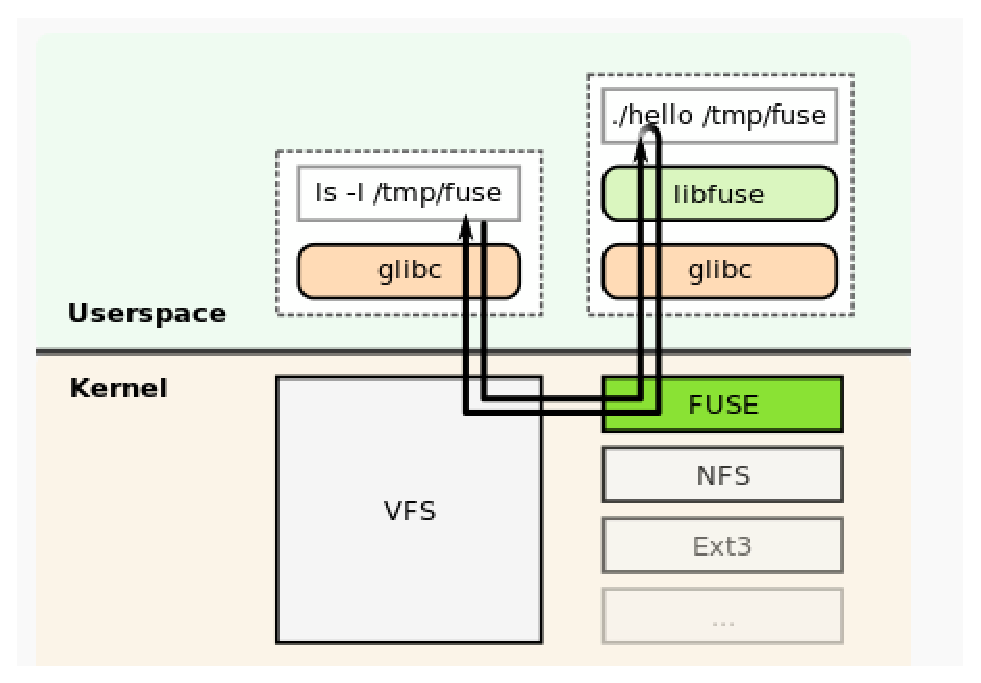
\includegraphics[height=6cm,
    angle=0]{./images/FUSE.eps}}
\caption{FUSE: flow-chart diagram}
\label{fig:FUSE}
\end{figure}

\subsection{VFS}

To support different file systems, Linux has a {\bf Virtual File System} (VFS)
layer. VFS describes the system's files in terms of {\bf superblocks} and inodes
in much the same way as the EXT2 file system uses superblocks and inodes
(Sect.\ref{sec:EXT2}).
As each file system is initialised, it registers itself with the VFS. The real
file systems are either built into the kernel itself or are built as loadable
modules. 

When a block device based file system is mounted, and this includes the root
file system, the VFS must read its superblock. The VFS keeps a list of the
mounted file systems in the system together with their VFS superblocks. Each VFS
superblock contains information and pointers to routines that perform particular
functions. 

Each VFS superblock contains a pointer to the first VFS inode on the file
system. For the root file system, this is the inode that represents the ``/''
directory. The VFS also keeps a cache of directory lookups so that the inodes
for frequently used directories can be quickly found.
\url{http://www.tldp.org/LDP/tlk/fs/filesystem.html}

All file systems, of whatever type, are mounted onto a directory and the files
of the mounted file system cover up the existing contents of that directory.
This directory is known as the mount directory or mount point. When the file
system is unmounted, the mount directory's own files are once again revealed.  


\subsection{FUSE}

One of the more recent directions in file system is to enable Filesystems
in User Space. It means that user can add support to new file system without
recompiling the O/S kernel. 

\chapter{Dedicated data server}

Typically, you can have one data server or multiple data servers.


Servers assigned roles: metadata, data, or both


\section{metadata server}
\label{sec:metadata-server}

Metadata server (MDS) stores directory and file metadata
(Sect.\ref{sec:metadata-in-a-block-oriented-filesystem}).
Often a single metadata server stores all metadata for file system.
